\section{Ranking Engines and Ground Truth}
\label{sec:4}

SaG ranks components with three kinds of engine. The \textbf{closed-form engine} \texttt{Topo-QoS} is QoS-weighted betweenness on the dependency projection, the training-free engine registered before the study (Section~\ref{sec:6.2}); training-free dependency counts on the same projection are evaluated beside it (Section~\ref{sec:6.2}). The \textbf{learned engines} are graph neural networks trained on the typed multigraph (this section); only the typed engine propagates information into the Application nodes it scores (Section~\ref{sec:6.2}). The \textbf{hybrid engines} are learned engines that correct the closed-form score (Section~\ref{sec:rq1-hybrid}). All are trained or scored against simulation oracles that run on a separate graph view (Sections~\ref{sec:4.3}--\ref{sec:4.4}). Figure~\ref{fig:engines} shows how the three engines relate and how they are evaluated. Full hyperparameters and training commands are on the experiment pages of the replication repository (Section~\ref{sec:6.1}).

\begin{figure}[htbp]
\centering
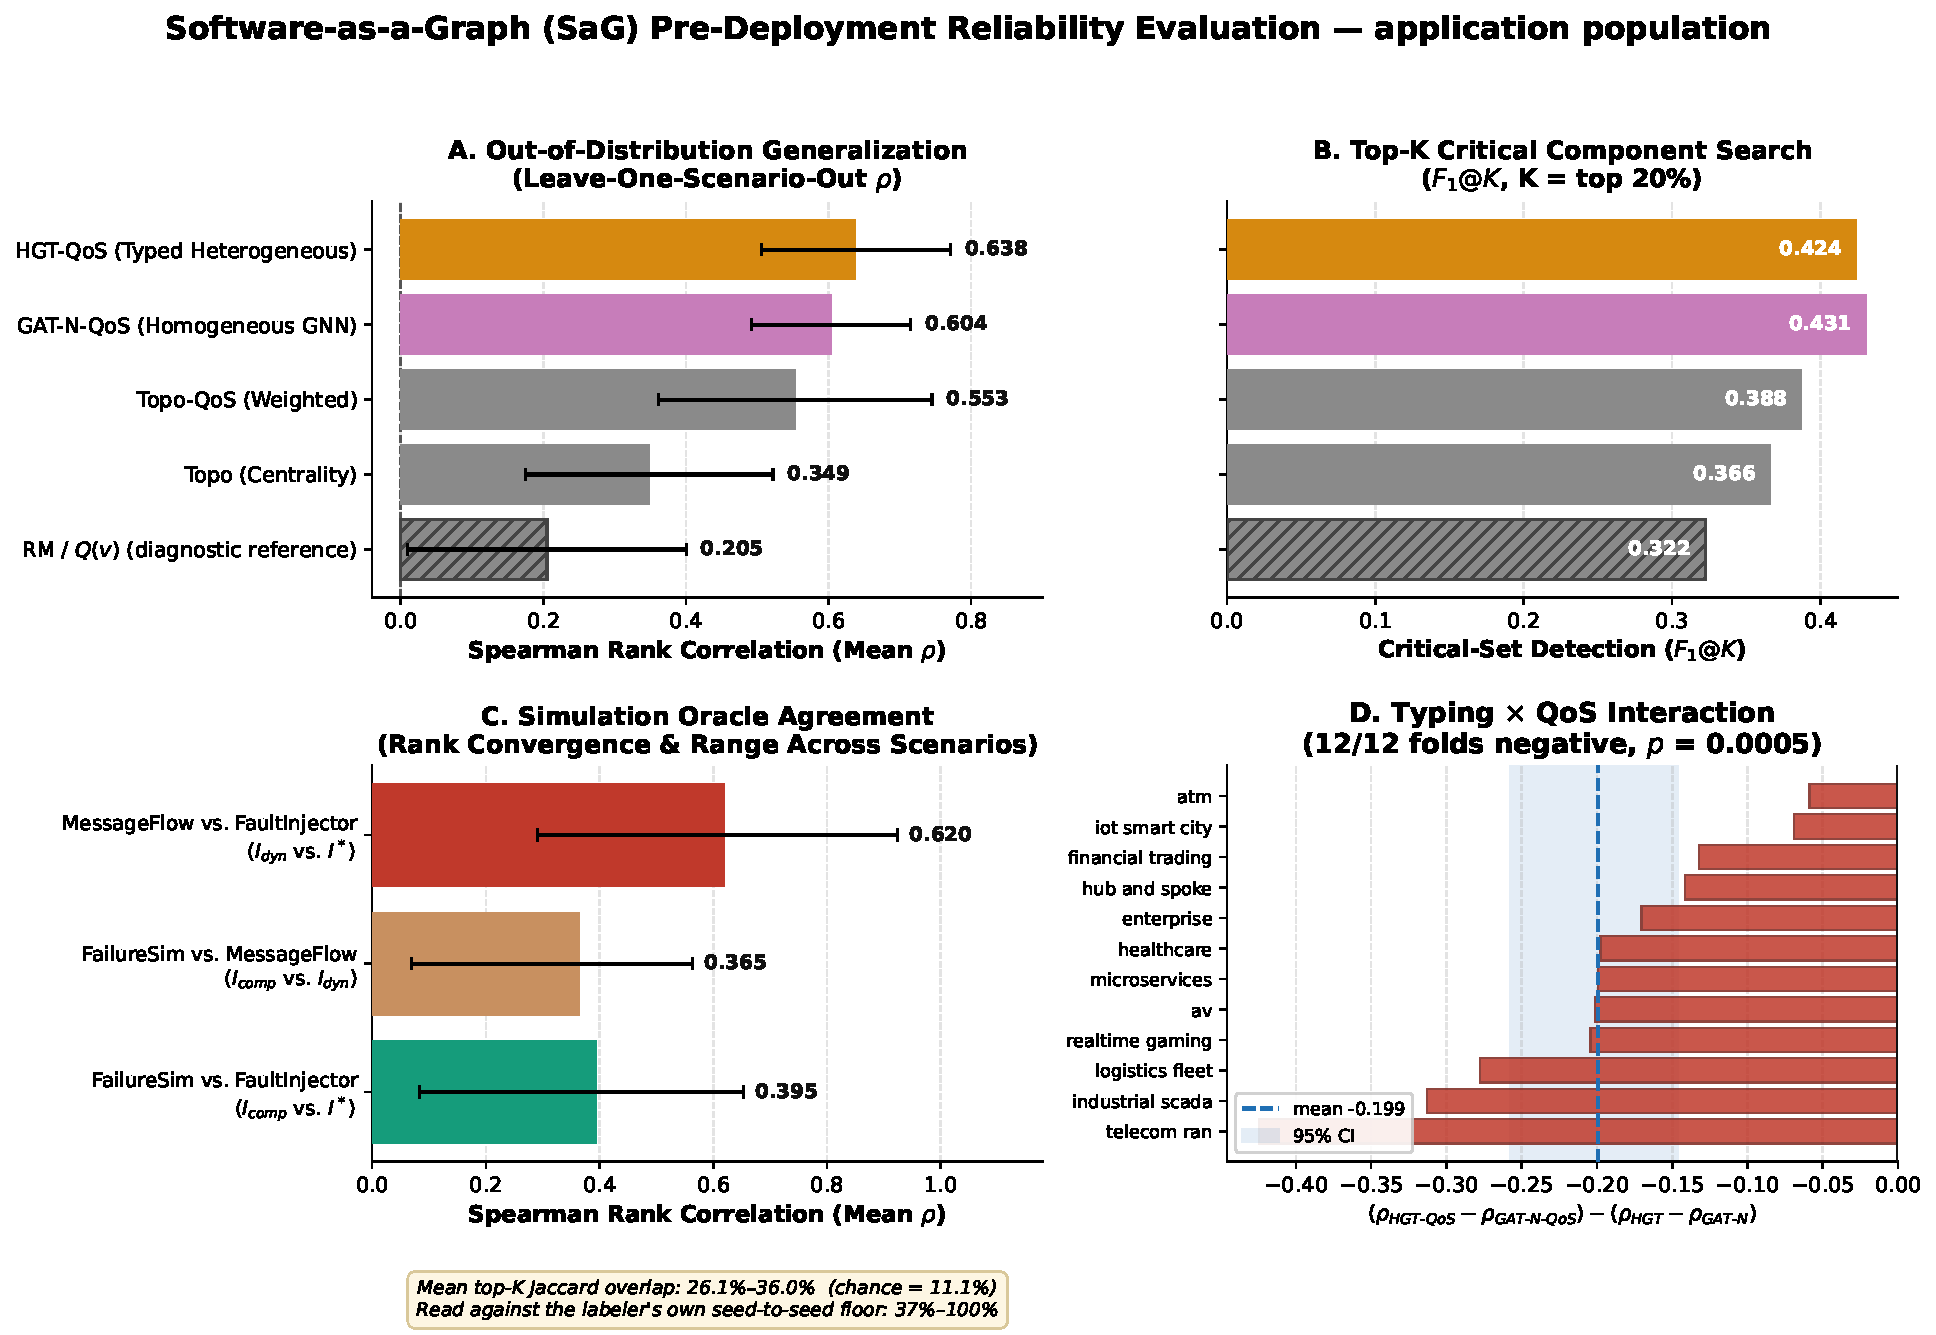
\includegraphics[width=\linewidth]{figures/Figure_3}
\caption{(a)~SaG's three ranking engines read the same analysis graph. The closed-form engine scores QoS-weighted betweenness $p(v)$; the learned engine outputs a logit $z(v)$. A hybrid engine gives the learned engine $p(v)$ as an extra input feature and adds a learned correction to it on the logit scale, $\sigma(z + \alpha\,\operatorname{logit} p)$, with one learnable scalar $\alpha$. (b)~Ground truth comes from simulation oracles on the structural graph, which no predictor reads. Engines are evaluated by leave-one-scenario-out cross-validation over twelve synthetic architectures (each row trains on eleven and tests on the held-out one) and zero-shot on five open-source system models.}
\label{fig:engines}
\end{figure}

\subsection{Heterogeneous Graph Transformer}
\label{sec:4.1}

The learned engine \texttt{HGT-QoS} is a three-layer Heterogeneous Graph Transformer (HGT) \cite{hu2020hgt} in PyTorch Geometric \cite{fey2019fast}, with hidden dimension $D = 64$ and $H = 4$ heads. Entity-specific projections map raw features $x_v \in \mathbb{R}^{19\text{--}25}$ (Section~\ref{sec:3.4}) into the hidden space, $h_v^{(0)} = \text{LayerNorm}(\text{GELU}(W_{\tau(v)} x_v))$. For each meta-relation $\langle \tau(u), \phi(e), \tau(v)\rangle$, attention uses type-parameterized keys $K(u) = h_u W_K^{\tau(u)}$, queries $Q(v) = \tilde{h}_v W_Q^{\tau(v)}$ and values $V(u) = h_u W_V^{\tau(u)}$, scaled by a learned per-meta-relation prior $\mu_{\langle \tau(u), \phi(e), \tau(v)\rangle}$. That prior is the relation-typing mechanism that RQ2 tests. Its input is the full typed multigraph of $G_{\text{analysis}}$: all five entity types and seven edge types, the six structural relations of Table~\ref{tab:1} together with the derived \texttt{DEPENDS\_ON} edges. Message passing runs over this graph and its transpose, to capture downstream starvation and upstream backpressure, with residual connections, dropout $0.10$ and layer normalization.

\subsubsection{QoS Edge Encoding (16-D)}
\label{sec:4.1.1}

Each directed edge carries a vector $e_{uv} \in \mathbb{R}^{16}$. Index 0 is the coupling weight $w_E(e)$ (Section~\ref{sec:3.2}), index 1 the normalized count of simple paths through $e$, indices 2--8 a one-hot of the seven relation types, and indices 9--15 the middleware QoS parameters on \texttt{PUBLISHES\_TO}/\texttt{SUBSCRIBES\_TO} edges, zero elsewhere. Six QoS dimensions are active in our corpus: reliability, durability, priority, a flag for edges whose QoS departs from the scenario's modal profile, and a deadline pair (active flag and log-deadline, populated on $463$ of $615$ topics). A seventh, max-blocking time, is reserved for hard real-time profiles and is zero throughout. The encoding is projected and added to the target representation before attention, $\tilde{h}_v = h_v + W_{\text{edge}} e_{uv}$.

\subsection{Prediction Head and Training Objective}
\label{sec:4.2}

A composite head predicts cascade impact, $\hat{I}^*(v) = \sigma(\text{MLP}_C(h_v \parallel \hat{a}_1(v) \parallel \hat{a}_2(v)))$. The two auxiliary heads $\hat{a}_1, \hat{a}_2$ act only as learned feature enrichment: $\hat{a}_1$ is supervised on $I^*$ and $\hat{a}_2$ is unsupervised. The optimized objective combines regression with listwise and pairwise ranking:
\begin{equation}
\label{eq:loss_active}
\mathcal{L} = \text{MSE}(\hat{I}^*, I^*) + 0.5 \cdot \text{MSE}(\hat{a}_1, I^*) + 0.3 \cdot \mathcal{L}_{\text{rank}} + 0.1 \cdot \mathcal{L}_{\text{pairwise}},
\end{equation}
where $\mathcal{L}_{\text{rank}}$ is ListMLE \cite{xia2008listwise} over the ground-truth permutation $\pi$,
\begin{equation}
\label{eq:listmle}
\mathcal{L}_{\text{rank}} = -\frac{1}{N}\sum_{i=1}^N \Big( \hat{s}_{\pi_i} - \log \sum_{j=i}^N \exp(\hat{s}_{\pi_j}) \Big),
\end{equation}
and $\mathcal{L}_{\text{pairwise}}$ is a margin-ranking loss ($\gamma = 0.05$) over pairs whose true impacts differ by more than $\gamma$. A general form with a maintainability term and a consistency term tying the heads to the explanation layer exists but is switched off throughout, so the learned engines and the explanation layer share no parameters (Supplementary Section~\ref{S-supp:objective}).

Models are trained with AdamW ($\eta = 3 \times 10^{-4}$, weight decay $10^{-4}$) under cosine warm restarts for up to 300 epochs, with early stopping at patience 30 on an inner validation split. Five seeds $\{42, 123, 456, 789, 2024\}$ are used throughout. Architectural hyperparameters follow conventional HGT values, and the loss coefficients were set by judgment. Neither was tuned on any evaluation split, so every learned arm is compared untuned.

\subsection{Ground-Truth Simulation Oracles}
\label{sec:4.3}

Ground truth comes from failure simulations over the raw structural multigraph $G_{\text{structural}}$. Table~\ref{tab:oracle_roles} summarizes the three oracles this study uses.

\begin{table}[htbp]
\centering
\footnotesize
\caption{Simulation oracles, operational constructs, and evaluation roles.}
\label{tab:oracle_roles}
\resizebox{\linewidth}{!}{%
\begin{tabular}{llll}
\toprule
\textbf{Oracle} & \textbf{Physical Mechanism} & \textbf{Nature} & \textbf{Role in Evaluation} \\
\midrule
$I^*(v)$ & Threshold cascade over topic feed loss + QoS ladder & Stochastic, 5 seeds & Primary ranking target (RQ1--RQ3) \\
$I_{\text{comp}}(v)$ & Severity mixture: reachability + fragmentation & Deterministic & Explanation layer / Validate gate \\
$I_{\text{dyn}}(v)$ & Discrete-event SimPy message queuing & Stochastic & Convergent-validity probe \\
\bottomrule
\end{tabular}%
}
\end{table}

\noindent\textbf{Primary target, $I^*(v)$.} The oracle crashes component $v$ and propagates the outage in waves until a fixpoint. In each wave, (i)~every dependent of a failed library fails outright, and (ii)~every topic's feed loss is recomputed as the larger of the rate-weighted share of its publishers that have failed and the share of its routing brokers that have failed. A subscriber's loss is the mean feed loss over its topics, scaled by a declared QoS severity ladder ($\times 1.2$ \texttt{RELIABLE}, $\times 1.15$ high priority, $\times 1.05$ medium) and clamped to $[0, 1]$. A subscriber whose loss reaches the propagation threshold $\theta = 0.2$ fails with probability $\min(1, \text{loss}/\theta) \cdot d_k$, where the damping $d_k = \max(0.25, 1 - 0.15k)$ decreases with wave $k$. $I^*(v)$ is the mean continuous loss over the intact graph's subscribers, averaged over five seeds that drive the Bernoulli draws and the propagation order. The ladder encodes severity rather than likelihood: a consumer that subscribes with reliable delivery or high priority is one that cannot tolerate missing samples, so the same loss harms it more.

\noindent\textbf{Robustness to the oracle's free parameters.} The shipped labels are stable under the oracle's own parameters. Re-labelling over $\theta \in \{0.1, 0.2, 0.3\}$ and damping steps $\{0.10, 0.15, 0.20\}$ keeps Application rankings at mean Spearman $0.86$--$0.99$ against the shipped setting, and moves the closed-form engine's accuracy only within $0.50$--$0.58$ (Supplementary Table~\ref{S-tab:a7-oracle}).

\noindent\textbf{How much QoS is in this label.} The ladder reads reliability and priority only, and disabling QoS scaling entirely leaves the Application ordering nearly intact: mean Spearman $\rho = 0.965$ against the ladder across the twelve folds (range $0.891$--$0.999$); substituting a durability-aware $w(t)$ scaling moves it less still ($\rho = 0.977$). The top-$K$ set is the sensitive construct: ladder and topology-only labels agree at mean Jaccard $0.678$, so QoS changes \emph{which} components are named critical rather than their order. $I^*$ is therefore a near-topological target, which bounds what any QoS encoding can be credited with on it (Sections~\ref{sec:rq1-qos} and~\ref{sec:rq2}).

\noindent\textbf{Further oracles.} $I_{\text{comp}}(v)$ is a severity-weighted mixture of reachability loss, fragmentation, throughput loss and flow disruption, with unswept AHP coefficients $(0.35, 0.25, 0.25, 0.15)$. It labels the explanation layer's evaluation and is never used for forecasting. $I_{\text{dyn}}(v)$ is a SimPy \cite{team2020simpy} message-flow simulation of emission rates, stochastic latencies and broker buffer saturation. It returns the drop in delivered message rate to surviving consumers and serves as an independent convergent-validity probe. It agrees with $I^*$ at $\rho = 0.627$, which is substantial but below $I^*$'s own seed-to-seed test--retest of $0.811$--$1.000$, so the two measure related but distinct constructs (Supplementary Section~\ref{S-supp:convergent}). Topic criticality is a predictor input, so it is masked out of every oracle's severity term. Results established against one oracle are never transferred to another.

\subsection{Input--Label Independence Guarantee}
\label{sec:4.4}

Features are built only from $G_{\text{analysis}}$: static topology, code metrics and declared QoS. Labels are computed only on $G_{\text{structural}}$ by the simulation oracles. No simulation output or runtime telemetry is exposed as a predictor input, and a CI test enforces the separation (\path{tests/test_independence_guarantee.py}). The guarantee is procedural: it rules out circular feature construction, not shared semantics. The oracle re-derives the same library and publish--subscribe dependency rules (Rules~1 and~5) from raw edges for its propagation step, and $I^*(v)$ is a reachability functional of the same architecture the predictors read. Ranking $I^*$ is therefore the task of recovering, from the dependency projection, how far each component's failure reaches, and simple counts over that projection are the natural first reference (Section~\ref{sec:6.2}).
